\documentclass[11pt,a4paper]{article}

\usepackage[a4paper,margin=1in]{geometry}
\usepackage{graphicx}
\usepackage{xcolor}
\usepackage{booktabs}
\usepackage{array}
\usepackage{longtable}
\usepackage{hyperref}
\usepackage{enumitem}
\usepackage{tikz}
\usetikzlibrary{arrows.meta,positioning,shapes.geometric}

\definecolor{navy}{HTML}{071426}
\definecolor{panel}{HTML}{10243D}
\definecolor{accent}{HTML}{38BDF8}
\definecolor{muted}{HTML}{64748B}

\hypersetup{
  colorlinks=true,
  linkcolor=navy,
  urlcolor=accent,
  citecolor=navy
}

\setlist[itemize]{topsep=4pt,itemsep=2pt,leftmargin=1.4em}
\setlist[enumerate]{topsep=4pt,itemsep=2pt,leftmargin=1.6em}

\newcommand{\tech}[1]{\texttt{#1}}
\newcommand{\sectionbreak}{\vspace{0.35em}}

\title{\textbf{SmartFetch: High-Level Report}\\
\large Adaptive Web Data Extraction Web Application}
\author{
Youssef Mabrouk \and Adam Hajri \and Jaouher Chouchane \and Mohammed Sanad\\
\small Information Assurance and Security
}
\date{May 2026}

\begin{document}

\maketitle

\begin{abstract}
SmartFetch is a client-server web application for adaptive web data extraction from one user-provided webpage at a time. The system accepts a public URL, retrieves and analyzes the HTML, suggests filters based on detected content, allows the user to select the desired data types, previews cleaned results, and exports the output as JSON or CSV. This report summarizes the purpose, scope, architecture, data flow, implementation, security controls, testing approach, and limitations of the final SmartFetch web application.
\end{abstract}

\tableofcontents
\newpage

\section{Introduction}

Manual collection of web data is slow, repetitive, and prone to errors. Websites also present information using different layouts and HTML structures, which means a scraper designed for one website can fail when the page structure changes. SmartFetch addresses this problem by analyzing the current webpage first and then generating extraction filters dynamically.

The project is intentionally limited to a single webpage supplied by the user. It is not a crawler and does not automatically follow links. This design keeps the application easier to control, safer to test, and realistic for the project scope.

\section{Project Objective}

The main objective of SmartFetch is to provide a controlled and adaptive data extraction workflow:

\begin{enumerate}
  \item Accept one public webpage URL from the user.
  \item Validate the URL and retrieve the page HTML.
  \item Analyze the HTML structure to detect available data types.
  \item Suggest relevant filters automatically.
  \item Extract only the data selected by the user.
  \item Clean the extracted output by trimming whitespace, removing empty values, and removing duplicates.
  \item Preview the results in the browser.
  \item Export the final result as JSON or CSV.
\end{enumerate}

\section{Scope}

SmartFetch focuses on adaptive extraction from one webpage at a time. It supports static HTML retrieval and parsing through the backend. The current system does not execute JavaScript on target websites, does not crawl multiple pages, and does not log into websites.

\begin{table}[h]
\centering
\begin{tabular}{p{0.45\linewidth}p{0.45\linewidth}}
\toprule
\textbf{Included in Scope} & \textbf{Outside Current Scope} \\
\midrule
Single public webpage analysis & Full-site crawling \\
HTML parsing with Cheerio & JavaScript-rendered page execution \\
Adaptive filter suggestions & Login or authenticated scraping \\
Preview and export as JSON/CSV & Scheduled or background scraping \\
Basic URL and SSRF protection & Proxy rotation or anti-bot bypassing \\
\bottomrule
\end{tabular}
\caption{SmartFetch scope boundaries.}
\end{table}

\section{Web Scraping Concepts}

A web scraper generally sends an HTTP request to a target website, receives HTML as the response, parses the HTML structure, extracts selected data, cleans the result, and stores or exports it in a structured format. SmartFetch uses these same concepts but avoids crawler behavior. Instead of discovering many pages, it processes only the URL entered by the user.

\section{Final Application Overview}

The final SmartFetch application provides a modern web interface with four main sections:

\begin{itemize}
  \item \textbf{URL Input:} the user enters the target webpage URL and starts analysis.
  \item \textbf{Suggested Filters:} the application displays available filters based on detected elements.
  \item \textbf{Preview:} extracted data is shown in a readable table or, for grouped mode, an optional card view.
  \item \textbf{Export:} the user downloads the latest extraction as JSON or CSV.
\end{itemize}

\begin{figure}[h]
\centering
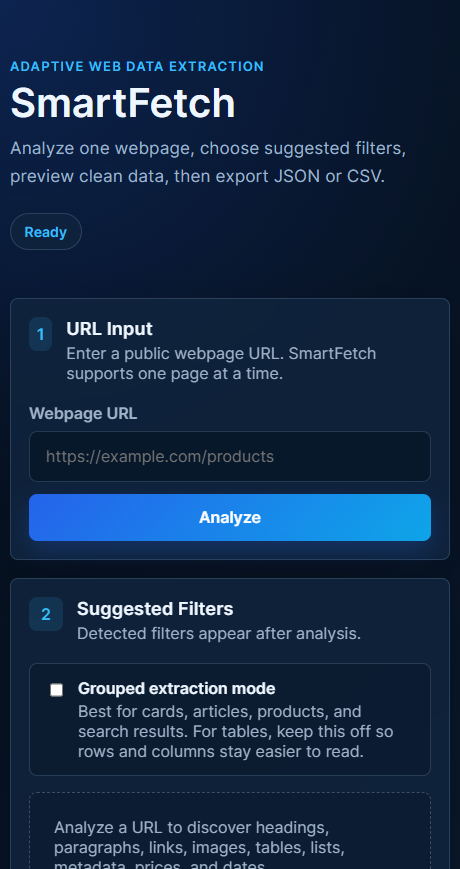
\includegraphics[width=0.95\linewidth]{assets/smartfetch-home.png}
\caption{SmartFetch web application interface.}
\end{figure}

\section{Technology Stack}

\begin{longtable}{p{0.25\linewidth}p{0.65\linewidth}}
\toprule
\textbf{Technology} & \textbf{Role in SmartFetch} \\
\midrule
\endhead
HTML & Defines the frontend page structure. \\
CSS & Provides the dark navy visual design, responsive layout, panels, buttons, and preview styling. \\
JavaScript & Handles frontend interactivity, API calls, filter selection, preview rendering, recent URL history, and downloads. \\
Node.js & Runs the backend server. \\
Express.js & Defines API routes and serves the static frontend. \\
Axios & Retrieves HTML from the target webpage with timeout and redirect handling. \\
Cheerio & Parses HTML on the backend and extracts elements using CSS selectors. \\
JSON & Used for API communication and export. \\
CSV & Used for spreadsheet-friendly export. \\
\bottomrule
\caption{Main implementation technologies.}
\end{longtable}

\section{High-Level Architecture}

SmartFetch follows a client-server architecture. The browser handles user interaction, while the backend performs validation, HTML retrieval, analysis, extraction, cleaning, and export preparation.

\begin{figure}[h]
\centering
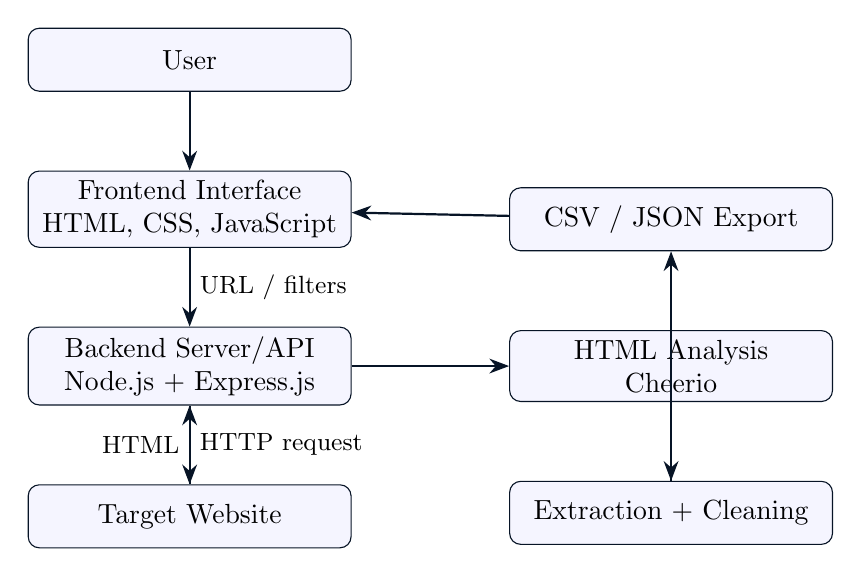
\begin{tikzpicture}[
  node distance=1.0cm,
  box/.style={draw=navy, rounded corners, fill=blue!4, minimum width=4.1cm, minimum height=0.8cm, align=center},
  arrow/.style={-{Stealth[length=2.5mm]}, thick, draw=navy}
]
\node[box] (user) {User};
\node[box, below=of user] (frontend) {Frontend Interface\\HTML, CSS, JavaScript};
\node[box, below=of frontend] (backend) {Backend Server/API\\Node.js + Express.js};
\node[box, below=of backend] (website) {Target Website};
\node[box, right=2.0cm of backend] (parser) {HTML Analysis\\Cheerio};
\node[box, below=of parser] (extractor) {Extraction + Cleaning};
\node[box, above=of parser] (export) {CSV / JSON Export};

\draw[arrow] (user) -- (frontend);
\draw[arrow] (frontend) -- node[right, font=\small] {URL / filters} (backend);
\draw[arrow] (backend) -- node[right, font=\small] {HTTP request} (website);
\draw[arrow] (website) -- node[left, font=\small] {HTML} (backend);
\draw[arrow] (backend) -- (parser);
\draw[arrow] (parser) -- (extractor);
\draw[arrow] (extractor) -- (export);
\draw[arrow] (export) -- (frontend);
\end{tikzpicture}
\caption{SmartFetch high-level architecture.}
\end{figure}

\section{System Flow}

The complete SmartFetch workflow is divided into analysis and extraction phases.

\begin{figure}[h]
\centering
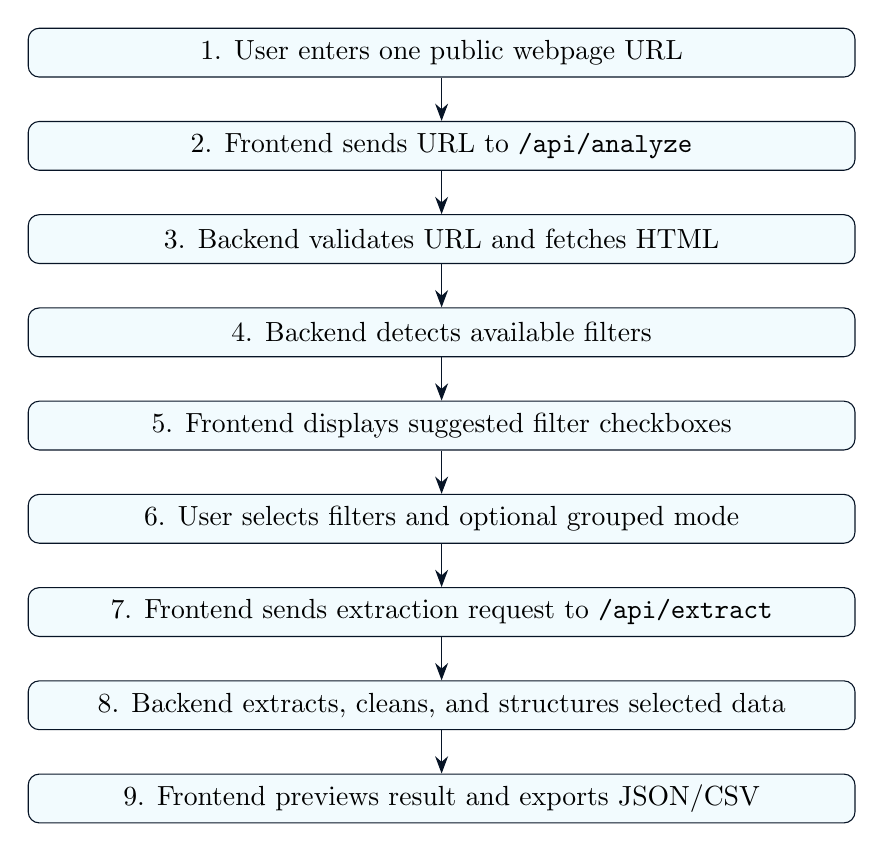
\begin{tikzpicture}[
  node distance=0.55cm,
  flowstep/.style={draw=navy, rounded corners, fill=cyan!5, minimum width=10.5cm, minimum height=0.62cm, align=center},
  arrow/.style={-{Stealth[length=2.2mm]}, draw=navy}
]
\node[flowstep] (s1) {1. User enters one public webpage URL};
\node[flowstep, below=of s1] (s2) {2. Frontend sends URL to \tech{/api/analyze}};
\node[flowstep, below=of s2] (s3) {3. Backend validates URL and fetches HTML};
\node[flowstep, below=of s3] (s4) {4. Backend detects available filters};
\node[flowstep, below=of s4] (s5) {5. Frontend displays suggested filter checkboxes};
\node[flowstep, below=of s5] (s6) {6. User selects filters and optional grouped mode};
\node[flowstep, below=of s6] (s7) {7. Frontend sends extraction request to \tech{/api/extract}};
\node[flowstep, below=of s7] (s8) {8. Backend extracts, cleans, and structures selected data};
\node[flowstep, below=of s8] (s9) {9. Frontend previews result and exports JSON/CSV};
\foreach \a/\b in {s1/s2,s2/s3,s3/s4,s4/s5,s5/s6,s6/s7,s7/s8,s8/s9}
  \draw[arrow] (\a) -- (\b);
\end{tikzpicture}
\caption{End-to-end SmartFetch workflow.}
\end{figure}

\section{API Design}

\subsection{Analyze Endpoint}

The \tech{POST /api/analyze} endpoint receives a URL, validates it, retrieves the webpage, parses the HTML, and returns the detected filters. The frontend uses this response to display selectable filter cards.

\subsection{Extract Endpoint}

The \tech{POST /api/extract} endpoint receives a URL, selected filters, and the grouped-mode option. It extracts the selected data, cleans the result, computes a summary, and returns structured sections plus a CSV string.

\begin{table}[h]
\centering
\begin{tabular}{p{0.22\linewidth}p{0.30\linewidth}p{0.36\linewidth}}
\toprule
\textbf{Endpoint} & \textbf{Input} & \textbf{Output} \\
\midrule
\tech{/api/analyze} & URL & Final URL, page title, suggested filters, counts \\
\tech{/api/extract} & URL, filters, grouped mode & Extracted sections, summary, export settings, CSV data \\
\bottomrule
\end{tabular}
\caption{SmartFetch API endpoints.}
\end{table}

\section{Adaptive Filters}

SmartFetch detects the following filters from the target HTML:

\begin{longtable}{p{0.22\linewidth}p{0.35\linewidth}p{0.33\linewidth}}
\toprule
\textbf{Filter} & \textbf{Detection Source} & \textbf{Extracted Data} \\
\midrule
\endhead
Headings & \tech{h1}, \tech{h2}, \tech{h3} & Level and text \\
Paragraphs & \tech{p} tags & Readable text content \\
Links & \tech{a[href]} & Link text and resolved URL \\
Images & \tech{img} & Image source and alt text \\
Tables & \tech{table}, \tech{tr}, \tech{th}, \tech{td}, and selected table-like rows & Row values and structured columns when possible \\
Lists & \tech{ul}, \tech{ol}, \tech{li} & List items grouped by list type \\
Metadata & \tech{title}, \tech{meta} tags & Title, description, keywords, Open Graph, and social metadata \\
Prices & Price-like text patterns & Values using symbols or formats such as \$, EUR, TND, and numeric price patterns \\
Dates & \tech{time}, \tech{datetime}, and date-like text & Date values from semantic tags and page text \\
\bottomrule
\caption{Detected SmartFetch filters.}
\end{longtable}

\section{Separate and Grouped Extraction Modes}

SmartFetch supports two extraction modes:

\begin{itemize}
  \item \textbf{Separate mode:} each selected filter is extracted independently. This is best for tables and when the user wants a simple list of one data type.
  \item \textbf{Grouped mode:} the backend attempts to preserve relationships between elements that appear inside the same card, article, product block, search result, or section. This is useful for pages where a heading, image, price, date, paragraph, and link belong to the same item.
\end{itemize}

Grouped extraction was added to better match real web layouts such as news cards, product listings, and repeated search results. The preview supports both table view and card view only when grouped mode is active.

\section{Data Cleaning}

Raw web data can include empty strings, repeated values, extra spaces, navigation links, footer links, or duplicated elements. SmartFetch applies cleaning before preview and export:

\begin{itemize}
  \item trims whitespace and normalizes repeated spaces;
  \item removes empty rows and empty values;
  \item removes duplicate rows;
  \item resolves relative URLs into absolute URLs;
  \item reduces noisy navigation, footer, account, cookie, and repeated site-wide links;
  \item deduplicates grouped links by destination URL;
  \item keeps image previews as thumbnails in the browser while exporting image URLs in JSON and CSV.
\end{itemize}

\section{Export Design}

SmartFetch provides two export formats:

\begin{itemize}
  \item \textbf{JSON export:} preserves the full response structure, including sections, selected filters, grouped mode, source URL, extraction duration, and extracted rows.
  \item \textbf{CSV export:} creates spreadsheet-friendly rows. The export begins with a small settings block containing the source URL, grouped-mode status, selected filters, total rows, and extraction duration.
\end{itemize}

For complex table data, the backend attempts to keep meaningful columns, such as month or change fields in table-like layouts. For images, exports store URLs rather than embedding binary image data.

\section{Security and Ethical Considerations}

SmartFetch is designed for public webpage data only. It should not be used to collect private, sensitive, or personally identifiable information. The implementation includes several basic protections:

\begin{itemize}
  \item rejects invalid URLs;
  \item allows only \tech{http} and \tech{https} protocols;
  \item blocks localhost and private IP address ranges where possible;
  \item validates redirects before following them;
  \item limits request duration with a timeout;
  \item limits HTML response size;
  \item processes one URL at a time instead of crawling many pages.
\end{itemize}

These controls reduce risk but do not replace responsible use. Users should respect website terms, robots policies, and request frequency limits.

\section{Testing Strategy}

The project includes automated backend tests using Node's built-in test runner. The tests cover:

\begin{itemize}
  \item whitespace normalization and duplicate removal;
  \item extraction of headings, links, images, tables, prices, dates, lists, and metadata;
  \item grouped extraction behavior;
  \item splitting large grouped wrappers into smaller cards;
  \item duplicate link removal in grouped mode;
  \item page-level date handling;
  \item table-like div extraction, including Steam-style hardware rows;
  \item CSV export with settings;
  \item private IP blocking and URL resolution.
\end{itemize}

At the time of this report, the test suite passes with 11 successful tests and 0 failures.

\section{Limitations}

SmartFetch is functional and ready for demonstration, but it still has realistic limitations:

\begin{itemize}
  \item it does not execute JavaScript on target websites, so content rendered after page load may not appear in the fetched HTML;
  \item grouped extraction uses heuristics, so very unusual layouts may produce imperfect grouping;
  \item it does not handle login-protected pages;
  \item it does not include custom user-defined CSS selectors;
  \item it is intentionally not a full crawler.
\end{itemize}

\section{Future Improvements}

Possible future improvements include:

\begin{itemize}
  \item optional browser automation for JavaScript-heavy websites;
  \item saved custom filter presets;
  \item more advanced repeated-block detection;
  \item controlled multi-page crawling with strict limits;
  \item richer export templates for specific domains such as products, news, or research data;
  \item a small in-app explanation panel for grouped mode and each filter.
\end{itemize}

\section{Conclusion}

SmartFetch successfully implements the high-level project design as a working web application. It combines a clean frontend interface with a backend analysis and extraction pipeline. The adaptive filter approach makes it more flexible than a fixed scraper, while the single-page scope and URL protections keep it controlled and suitable for academic demonstration. The final application supports analysis, extraction, preview, grouped mode, data cleaning, and JSON/CSV export, fulfilling the main objectives described in the project documents.

\end{document}
